\section{The Additional Variables of Kent's Theory}\label{additional}
The second similarity Kent's theory has with the Bohmian interpretation is that it posits the reality of some additional variables beyond standard quantum theory (i.e. in addition to the quantum state\footnote{We may wish to think of these additional variables as hidden variables, but we are not obliged to since we don't speculate on whether these additional variables are necessarily unknowable. Rather, we just see them as supplementing the quantum state so as to provide a complete description of the system.}). Some details in the section are rather technical, so I've split this section into two subsections: the first section gives an overview, and the second section is more technical and can be skipped if desired. 
\subsection{Overview}\label{additionalOverview}
In the Bohmian interpretation, the additional variables are the positions and momenta of all the particles, whereas in Kent's theory, the additional variables specify the mass-energy density on a three-dimensional distant future spacelike hypersurface $S$  %
\nomenclature{$S$}{A distant future hypersurface on which a notional energy-density measurement is made, \nomrefpage}%
 in spacetime. 

To describe what is meant by a three-dimensional hyperspace $S$, we will need some terminology and notation that is used in special relativity. A \textbf{spacetime location}\index{spacetime location}\label{spacetimedef} is a point $(x^1,x^2,x^3)$ in three-dimensional space at a particular instant of time $t$, and hence described by four numbers $(x^0,x^1,x^2,x^3)$  %
\nomenclature{$(x^0,x^1,x^2,x^3)$}{A spacetime location, \nomrefpage}%
where $x^0=c t$  %
\nomenclature{$x^0$}{$x^0=c t$, \nomrefpage}%
 and where $c$ is the speed of light.\footnote{Multiplying time by the speed of light means that $x^0$ is a distance like $x^1,x^2$, and $x^3$. } We will use the convention of boldface type to depict spatial locations, e.g. $\bm{x}=(x^1,x^2,x^3)$,  %
 \nomenclature{$\bm{x}$}{A spatial location $(x^1,x^2,x^3)$, \nomrefpage}%
  and non-boldface type to depict a spacetime location, e.g. $x=(x^0,x^1,x^2,x^3)$.  %
  \nomenclature{$x$}{a spacetime location $(x^0,x^1,x^2,x^3)$, \nomrefpage}%

Now a key insight of special relativity is that there is no such thing as absolute time. So for instance, two spacetime locations might seem to be simultaneous from one frame of reference, but another person travelling at a different velocity would judge with equal propriety the same two spacetime locations to be non-simultaneous. But it is not the case that for any two spacetime locations we can always find a frame of reference in which the two spacetime locations are simultaneous -- sometimes this is not possible. We refer to distinct spacetime locations that could be simultaneous in some frame of references as being \textbf{spacelike-separated}\index{spacelike-separation}. For example, the two spacetime locations $o$ and $a$  in figure \ref{cone} are spacelike-separated. 

\begin{figure}[!h]
\centering

 \tikzset{surface/.style={draw=blue!70!black, fill=yellow!20!white, fill opacity=.6}}

 \newcommand{\coneback}[4][]{
 \draw[canvas is xy plane at z=#2, #1] (45-#4:#3) arc (45-#4:225+#4:#3) -- (O) --cycle;
 }
 \newcommand{\conefront}[4][]{
 \draw[canvas is xy plane at z=#2, #1] (45-#4:#3) arc (45-#4:-135+#4:#3) -- (O) --cycle;
 }
 \begin{tikzpicture}[tdplot_main_coords, grid/.style={help lines,violet!40!white,opacity=0.5},scale=1.25]
  \coordinate (O) at (0,0,0);
  
     \coneback[surface]{-3}{2}{-12}
   \conefront[surface]{-3}{2}{-12} 
  
   \fill[brown!40!white,opacity=0.5] (-4,-4,0) -- (-4,4,0) -- (4,4,0) -- (4,-4,0) -- cycle;
  
   \foreach \x in {-4,...,4}
     \foreach \y in {-4,...,4}
     {
         \draw[grid] (\x,-4) -- (\x,4);
         \draw[grid] (-4,\y) -- (4,\y);
         \draw[violet] (-4,4)--(-4,-4)--(4,-4)--(4,4)--cycle;
     }

   \draw[->] (-4,0,0) -- (4,0,0) {};
   \draw[->] (0,-4,0) -- (0,4,0) {};
   \coneback[surface]{3}{2}{12}
   \draw[-,dashed] (0,0,-2.65) -- (0,0,2.65) node[above] {};
   \draw[-,dashed] (0,0,-4) -- (0,0,-3.35) node[above] {};
   \draw[->,dashed] (0,0,3.35) -- (0,0,4) node[above] {time};
   \conefront[surface]{3}{2}{12}

   \draw[red, thick] (0,0,0) -- (4,0,2) node[below, pos=0.6, rotate=26.5651,scale=0.80,black] {spacelike-separated};
   \draw[red, thick] (0,0,0) -- (1.56,0.6,2.4) node[below, pos=0.62, rotate=55.1459,scale=0.80,black] {lightlike-separated};
   \draw[red, thick] (0,0,0) -- (-0.5,-0.85,2.2) node[above, pos=0.57, rotate=-65.8557,scale=0.80,black] {timelike-separated};
   \node[black] at (0,0,3) {Future Light Cone};
   \node[black] at (0,0,-3) {Past Light Cone};
   
   \fill (4,0,2) circle (2pt) node[above right] {$a$};
   \fill (0,0,0) circle (2pt) node[below ] {$o$};
   \fill (-0.5,-0.85,2.2) circle (2pt) node[above left] {$c$};
   \fill (1.56,0.6,2.4) circle (2pt) node[above left] {$b$};
  
   \node[black] at (0,4.7,0) {space};
   \node[black] at (5,-0.3,0) {space};
 \end{tikzpicture}
 \caption[Meaning of spacelike, timelike and lightlike-separation]{The meaning of spacelike, timelike and lightlike-separation when there are two space dimensions and one time dimension.}
 \label{cone}
\end{figure}
There are also distinct spacetime locations in spacetime that could be connected by a beam of light such as the two spacetime locations $o$ and $b$ in figure \ref{cone}. Such spacetime locations are referred to as being \textbf{lightlike-separated}\index{lightlike-separation}. For any given spacetime location, the spacetime locations that are lightlike-separated from it form two cones\footnote{Strictly speaking, the set of spacetime locations that are lightlike-separated from a given spacetime location form the surface of a cone rather than a cone (which is a convex object). But among physicists, the terminology light cone has stuck.} called the future light cone and the past light cone as shown in figure \ref{cone}. Because light appears to travel at the same speed no matter what frame of reference one uses, the light cone of a spacetime location remains invariant when one changes from one reference frame to another. In other words, if another spacetime location lies on the light cone of a spacetime location in one frame of reference, then it must lie on the light cone of this spacetime location in every frame of reference. 

Figure \ref{cone} also depicts two spacetime locations $o$ and $c$ that are \textbf{timelike-separated}\index{timelike-separation}. Such spacetime locations lie within the light cones of each other, and when two spacetime locations are timelike-separated, it is always possible to choose a frame of reference in which the two spacetime locations are located at the same point in space, but with one spacetime location occuring after the other  depending on which spacetime location is in  the future light cone of the other. 

Now a three-dimensional spacelike hypersurface $S$ in spacetime is a maximal\footnote{That is, it cannot be extended any further along any of its three dimensions, so it is not a small local surface contained within a boundary.} three-dimensional surface in which any two spacetime locations of $S$ are spacelike-separated. In this dissertation, we will assume that all hypersurfaces are spacelike and maximal.
Kent assumes that the hypersurface $S$ is in the distant future of an expanding universe so that nearly all the particles that can decay have already done so, and that all the particles that are not bound together are very far from each other so that the probability of any particle collisions is very small. In other words, all the interesting physics in the universe has played its course before $S$.

At every spacetime location $x\in S$, there is a quantity $T_S(x)$\label{firstTS}  
called the \label{massenergydensity}\textbf{mass-energy density}\index{mass-energy density}.\footnote{The definition of $T_S(x)$ will be discussed in section \ref{massenergydensity}.} The important thing to note about $T_S(x)$ is that it does not depend on which frame of reference one is in.\footnote{The reason for why this is will be discussed in section \ref{massenergydensity}.}
  This property is in contrast to many physical properties that do depend on which frame of reference one is in. For example, the kinetic energy of an object will depend on the calculated velocity of the object, and this velocity will in turn depend on the frame of reference in which this calculation is done. 

Now Kent supposes that a notional measurement is made over the whole of $S$ to determine a measurement outcome for $T_S(x)$ which we denote as $\tau_S(x)$ for every $x\in S$.  It is these $\tau_S(x)$ that are the additional variables of his theory. How this determination of $T_S(x)$ comes about is up to one's philosophical preferences. For example, one could suppose that it was simply by divine fiat that this determination  of $T_S(x)$ comes about.\footnote{I will discuss my philosophical preference in the final chapter.} 
 %
 \nomenclature{$\tau_S(x)$}{A real valued function which specifies the outcome of the notional measurement $T_S(x)$ for every $x\in S$, \nomrefpage}%
 

{\interfootnotelinepenalty=10000 Clearly,  Kent is not assuming that such a measurement could be performed on $S$ in reality, hence his reason for referring to the measurement as fictitious/notional.\footnote{Kent uses the word fictitious when referring to these measurements, e.g. \cite[3]{Kent2014}. Butterfield refers to these measurements as notional e.g. \cite[17]{Butterfield}.} However, Kent does seem to be saying that there would be a fact of the matter about what value $T_S(x)$ would have approximately had at each $x\in S$ if it had been measured.\footnote{\label{asymptoticfootnote}Kent talks about taking the asymptotic limit as $S$ tends to the infinite future of $S_0$. In saying this, he supposes that the physics we are interested in happens between two hypersurfaces $S_0$ and $S_1$. Then given some measurement outcome $\tau_S$ on a hypersurface $S$ after $S_1$, for every hypersurface $S'$ after $S$, there is a range of possible measurements $\tau_{S'}$ on $S'$ that together occur with approximately the same probability as the measurement outcome of $\tau_S$ on $S$ and such that the beables between $S_0$ and $S_1$ determined by any one of the $\tau_S'$ outcomes on $S'$ in this range would be approximately the same as the beables determined by $\tau_S$ on $S$. See \cite[3]{Kent2014}.} Given that there is some fact of the matter about the value $\tau_S(x)$ that $T_S(x)$ takes for every $x\in S$ were $T_S(x)$ to be measured, Kent constructs a picture of physical reality that evolves in a way that is consistent with $T_S(x)$ being $\tau_S(x)$ for $x\in S$.} 

Kent's proposal might initially sound like he is suggesting that physical reality evolves unitarily from an initial state of the universe $\ket*{\Psi_0}$\label{Psi0PsiSdef} describing a hypersurface $S_0$ to a state $\ket*{\Psi_S}$ describing the hypersurface $S$, and then a measurement of $T_S(x)$ is made yielding a value $\tau_S(x)$ for all $x\in S$ which in turn  changes the past by a process of backwards causality so that the history of the universe evolving from $S_0$ is now consistent with $T_S(x)$ having the determinate value $\tau_S(x)$. However, it is not necessary to think that Kent's interpretation requires backwards causality. Rather, we can think of the values $\tau_S(x)$ for $T_S(x)$ as being determined primordially before the evolution of physical reality begins. In other words, we first suppose that the universe is initially in a determinate state $\ket*{\Psi_0}$ that describes a hypersurface $S_0$. Given this state, there are many possibilities for the measurement outcome $T_S(x)$ on the distant future hypersurface $S$ that can be worked out from $\ket*{\Psi_S}$, but we don't consider $\ket*{\Psi_S}$ as describing the state of actuality of the hypersurface $S$ -- all $\ket*{\Psi_S}$ does is describe possibilities. One of the possible outcomes $\tau_S(x)$ is then selected,\footnote{Kent doesn't say anything about the selection of $\tau_S(x)$ beyond its selection being consistent with the Born Rule.} and then physical reality evolves in a way that is consistent with $T_S(x)$ being $\tau_S(x)$ if a measurement were to be made on $S$. One can therefore avoid positing the need for backwards causality by insisting that the states that unitarily evolve from $S_0$ don't describe the actual state of the universe. Rather, there is just one history,\footnote{The role that $\tau_S(x)$ plays in determining this one history will be described in sections \ref{OneWorldFeature} and  \ref{kentcalculation}.} and this history is consistent with $T_S(x)$ being $\tau_S(x)$ for $x\in S$.

Now we saw on page \pageref{eigendef}, that for any measurement on a physical system, we can associate an observable whose eigenstates describe a possible state of the physical system in which the measurement is given by the observable's corresponding eigenvalue. Now in the case of the notional measurement of $T_S(x)$, there will be lots of observables, denoted by $\hat{T}_S(x)$, corresponding to all the different places $x\in S$ where the measurement could be made. Therefore, if a measurement were made on $S$ for all $x\in S$, the corresponding state of $S$ would not just be an eigenstate of one observable $\hat{T}_S(x)$,\label{firstHatTS} 
but rather, it would have to be an eigenstate of every observable $\hat{T}_S(x)$ for every $x\in S$. We will therefore need to speak of simultaneous $\hat{T}_S$-eigenstates and simultaneous $\hat{T}_S$-eigenvalues in order to specify the quantum state of $S$ on which $T_S(x)$ has a determinate value of $\tau_S(x)$ for every $x\in S$. This terminology will be described in more detail on page \pageref{simultaneous}.  Given that there is such a simultaneous $\hat{T}_S$-eigenstate, we can then work out via the Born Rule the probability this state would be selected given the initial state of the universe.

\subsection{Technical Details\textsuperscript{*}}\label{AdditionalVariablesDetails}  
In order to specify more precisely the additional variables that Kent's theory requires, we need to discuss the Tomonaga-Schwinger picture of relativistic quantum physics.\footnote{See \cite{SchwingerJulianI}; \cite{TomonagaI}} In order to explain this formulation, it is helpful to first consider  the distinction between the Heisenberg picture and the Schr\"{o}dinger picture of standard quantum theory. 

{\interfootnotelinepenalty=10000 In the \textbf{Heisenberg picture}\index{Heisenberg picture}, the states describing a system do not change over time. Rather, the observables change over time. So for instance, if there is a time-independent state $\ket*{\Phi}$ describing a system and there is some measurable quantity whose expectation value we wish to know at time $t$ given the state $\ket*{\Phi}$, %
\nomenclature{$\ket*{\Phi}$}{A state in the Heisenberg picture, \nomrefpage}%
 then we will need a time dependent observable $\hat{\bm{O}}(t)$,\footnote{See footnote \ref{boldref} for an explanation of the convention of using a boldface font for this observable.} say, corresponding to the measurable quantity at time $t$ from which we can calculate the expectation value $\ev*{\hat{\bm{O}}(t)}{\Phi}$ at time $t$  given the system is in state $\ket*{\Phi}$. In the context of quantum field theory, any observable $\hat{\bm{O}}(t)$ %
 \nomenclature{$\hat{\bm{O}}(t)$}{A time dependent observable in the Heisenberg picture, \nomrefpage}%
  in the Heisenberg picture will be expressible as a sum (or integral) of observables of the form $\hat{\bm{O}}(t, \bm{x})$, where $\hat{\bm{O}}(t, \bm{x})$ %
  \nomenclature{$\hat{\bm{O}}(t, \bm{x})$}{An observable in the Heisenberg picture at a particular time $t$ and spatial location $\bm{x}$, \nomrefpage}%
   is an observable of some quantity at a particular time $t$ and spatial location $\bm{x}$.\footnote{For example, in quantum electrodynamics (which is one kind of quantum field theory), the observables will be expressible in terms of fields such as the \emph{four-vector potential}\index{four-vector potential}  $A^\mu(x)$  %
   \nomenclature{$A^\mu(x)$}{The four-vector potential of the electromagnetic field, \nomrefpage}%  
   and the bispinor field $\psi(x)$ %
   \nomenclature{$\psi(x)$}{The bispinor field of quantum field theory, \nomrefpage}%  
    which are defined at all spacetime locations $(t, \bm{x})=(t, x^1, x^2, x^3)$. The four-vector potential $A^\mu(x)$ can be used to determine the electromagnetic field, and the bispinor field $\psi(x)$ can be used to determine the electric current density. In the Heisenberg picture, these fields will have corresponding Hilbert space operators at each spacetime location $x$ from which expectation values can be calculated at the spacetime location $x$ for a given time-independent state.}
\strut \\[\baselineskip]
The Heisenberg picture is contrasted with the \textbf{Schr\"{o}dinger picture}\index{Schr\"{o}dinger picture} in which the observables do not change over time, but rather the states change over time. So for instance, if there is a time-dependent state $\ket*{\Phi(t)}$}  %
\nomenclature{$\ket*{\Phi(t)}$}{Time dependent state in the Schr\"{o}dinger picture, \nomrefpage}%
 describing a system at a specific time $t$ and there is some measurable quantity whose expectation value we wish to know at time $t$ given the state $\ket*{\Phi(t)}$, then we will only require a time-independent observable $\hat{\bm{O}}$, %
 \nomenclature{$\hat{\bm{O}}$}{Time independent observable in the Schr\"{o}dinger picture, \nomrefpage}%
  say, corresponding to the measurable quantity from which we can calculate the expectation value $\ev*{\hat{\bm{O}}}{\Phi(t)}$. As in the Heisenberg picture, we can introduce a spatial dependence into the observables so that any observable  $\hat{\bm{O}}$ is expressible as a sum (or integral) of observables of the form $\hat{\bm{O}}(\bm{x})$  %
  \nomenclature{$\hat{\bm{O}}(\bm{x})$}{Spatial dependent but time independent observable in the Schr\"{o}dinger picture, \nomrefpage}%
  where $\hat{\bm{O}}(\bm{x})$ is an observable of some quantity at a particular spatial location $\bm{x}$.
\strut \\[\baselineskip] 
Now despite the Schr\"{o}dinger and Heisenberg pictures taking these different perspectives, they are nevertheless physically equivalent. This is because in both pictures, there is a unitary operator $U(\Delta t)$  %
\nomenclature{$U(\Delta t)$}{Unitary operator parameterized by a time interval $\Delta t$, \nomrefpage}%
for any time interval $\Delta t$ such that $U(\Delta t)\ket*{\Phi(t)}=\ket*{\Phi(t+\Delta t)}$, and $U(\Delta t)\hat{\bm{O}}(t, \bm{x})U(\Delta t)^{-1}=\hat{\bm{O}}(t+\Delta t, \bm{x})$. Thus, given the Schr\"{o}dinger picture, to get the Heisenberg picture, all we need to do is the following: firstly, we fix a time $t_0$ and let all the states of the form $\ket*{\Phi(t_0)}$ at time $t_0$ in the Schr\"{o}dinger picture be the state space for the Heisenberg picture; then for any Schr\"{o}dinger picture observable $\hat{\bm{O}}(\bm{x})$, we define the corresponding Heisenberg picture time-dependent observable 
\begin{equation*}
\hat{\bm{O}}(t, \bm{x})=U(t-t_0)\hat{\bm{O}}(\bm{x})U(t-t_0)^{-1}.
\end{equation*} 
Conversely, to move from the Heisenberg picture to the Schr\"{o}dinger, we first fix a reference time $t_0$. Then for any state $\ket*{\Phi}$ and observable $\hat{\bm{O}}(\bm{x})\myeq\hat{\bm{O}}(t, \bm{x})$ in the Heisenberg picture, the corresponding Schr\"{o}dinger picture time-dependent state at time $t$ will be $U(t-t_0)\ket*{\Phi}$, and the corresponding Schr\"{o}dinger picture time-independent observable will be $\hat{\bm{O}}(t_0, \bm{x})$.\footnote{Note that if there is a non-unitary aspect to the evolution of the Schr\"{o}dinger picture time-dependent state $\ket*{\Phi(t)}$ (such as would be the case if there was a collapse), then we can't expect the Schr\"{o}dinger picture and the Heisenberg picture to be equivalent. This is because there could be many different states that could evolve to $\ket*{\Phi(t)}$ if collapses are permitted, and so we wouldn't expect there to be an invertible operator $U(\Delta t)$ in terms of which we could define the Heisenberg picture observable  $\hat{\bm{O}}(t, \bm{x})$.  }

Now if there is a quantity we wish to measure at time $t_0$ with corresponding observable $\hat{\bm{O}}(\bm{x})\myeq\hat{\bm{O}}(t_0, \bm{x})$, then in both pictures, the expectation value of this measurable quantity given $\ket*{\Phi}\myeq\ket*{\Phi(t_0)}$ will be 
\begin{equation}\label{heisshrodeq}
  \ev*{\hat{\bm{O}}(\bm{x})}{\Phi(t_0)}=\ev*{\hat{\bm{O}}(t_0,\bm{x})}{\Phi(t_0)}=\ev*{\hat{\bm{O}}(t_0, \bm{x})}{\Phi}
\end{equation}
Since the left-hand side of (\ref{heisshrodeq}) is the Schr\"{o}dinger picture expectation value of $\hat{\bm{O}}(\bm{x})$, and the right-hand side of (\ref{heisshrodeq}) is the Heisenberg picture expectation value of $\hat{\bm{O}}(t_0,\bm{x})$, it follows that whatever picture we choose, it will make no difference to the calculated expectation values of observables -- in other words, the two pictures are physically equivalent.

Now although it is easy to move between both the Schr\"{o}dinger and Heisenberg pictures, they both give a privileged status to hypersurfaces of the form $t=\text{const}$. However, according to special relativity, there are no privileged hypersurfaces. One of the advantages of the Tomonaga-Schwinger picture is that it gives no privileged status to any class of hypersurfaces, but rather all hypersurfaces are placed on the same footing. We are going to see that the expectation value $\ev*{\hat{\bm{O}}(t_0,\bm{x})}{\Phi(t_0)}$  of equation (\ref{heisshrodeq}) is a special case of what Tomonaga and Schwinger consider more generally. 

We first note that if we can calculate $\ev*{\hat{\bm{O}}(t_0,\bm{x})}{\Phi(t_0)}$ for any $t_0$ and any $\bm{x}$, then we can calculate all the expectation values that might interest us. But we also note that in the expectation value $\ev*{\hat{\bm{O}}(t_0,\bm{x})}{\Phi(t_0)}$,  the $\ket*{\Phi(t_0)}$-state is the state of a hypersurface $t=t_0$, and $(t_0,\bm{x})$ is a spacetime location on this hypersurface. Now if we are to place all hypersurfaces on the same footing, then in specifying expectation values, we should be just as content in specifying expectation values of the form $\ev*{\hat{O}(x)}{\Psi[S]}$, where $S$ is any hypersurface, $\ket*{\Psi[S]}$ %
\nomenclature{$\ket*{\Psi[S]}$}{Hypersurface dependent state in the Tomonaga-Schwinger picture, \nomrefpage}% 
is any state of this hypersurface,\footnote{The convention of using square brackets such as in $\ket*{\Psi[S]}$ indicates that the thing in question is a \emph{functional}\index{functional}. Functions and functionals are closely related. A function $f$ is a mapping from one set (the domain) to another set (the codomain), such that each input yields a single output. The typical convention is to use round brackets to denote the output, e.g. $f(x)$ where $x$ is the input. A functional $g$, on the other hand, is a function that maps a space of functions or other mathematical objects (such as surfaces or volumes) to some value. The typical convention is to use square brackets to denote the output, e.g. $g[y]$ where $y$ is the input function or other mathematical object. So in the present case, $\ket*{\Phi[\cdot]}$ is a functional that takes a surface $S$ as input to produce a state $\ket*{\Phi[S]}$ as output.} $x$ is any spacetime location on the hypersurface $S$, and where $\hat{O}(x)$ %
\nomenclature{$\hat{O}(x)$}{Observable for any $x\in S$ in the Tomonaga-Schwinger picture, see equation (\ref{tsobservable}), \nomrefpage}%
 is any observable of $S$.\footnote{\label{boldref}Here I am following the convention of Schwinger of always using non-boldface type to indicate Tomonaga-Schwinger picture observables, and boldface type to indicate Heisenberg picture and Schr\"{o}dinger picture observables. See \cite[p. 1448]{SchwingerJulianI}.} The Tomonaga-Schwinger picture thus works with states of the form $\ket*{\Psi[S]}$ for any hypersurface $S$, and observables of the form $\hat{O}(x)$ with $x\in S$ acting on the state space of the hypersurface $S$ from which one can calculate the expectation value $\ev*{\hat{O}(x)}{\Psi[S]}$.

In order to construct $\ket*{\Psi[S]}$ and $\hat{O}(x)$, Schwinger introduces a unitary operator\footnote{See \cite[p. 1448]{SchwingerJulianI}.} $U[S]$ \label{SchwingerOperator}  %
\nomenclature{$U[S]$}{Unitary operator that maps the Heisenberg picture state $\ket*{\Phi}$ to the corresponding $\ket*{\Psi[S]}$-state that describes the state of the hypersurface $S$, i.e. $\ket*{\Psi[S]}=U[S]\ket*{\Phi}$ in the Tomonaga-Schwinger picture, \nomrefpage}%
that maps the $\ket*{\Phi}$-state of the Heisenberg picture to the corresponding $\ket*{\Psi[S]}$-state that describes the state of the hypersurface $S$, i.e. $\ket*{\Psi[S]}=U[S]\ket*{\Phi}$. Schwinger then defines the observable  
\begin{equation}\label{tsobservable}
  \hat{O}(x)=U[S]\hat{\bm{O}}(x)U[S]^{-1}
\end{equation}
on $S$ where $x$ is any spacetime location on $S$, and where $\hat{\bm{O}}(x)$ is any Heisenberg picture observable. Ostensibly, $\hat{O}(x)$ depends on the surface $S$,  but Schwinger shows that under conditions that are readily satisfied, $\hat{O}(x)$ is independent of the hypersurface $S$.\footnote{
  The required condition is that 
  \begin{equation*}
i\hbar\fdv{U[S]}{S(x)}=\mathcal{H}(x)U[S] 
\end{equation*}
  where $\mathcal{H}(x)$ is a Hermitian operator that is a Lorentz invariant function of the field quantities at the spacetime location $x$ and has the dimensions of an energy density, and where the \emph{functional derivative}\index{functional derivative} $U[S]$ is given by
  \begin{equation}\label{fddef}
  \fdv{U[S]}{S(x)}=\lim_{\delta \omega\rightarrow 0}\frac{U[S']-U[S]}{\delta\omega}
  \end{equation}%
  \nomenclature{$\fdv{U[S]}{S(x)}$}{Functional derivative, see equation (\ref{fddef}), \nomrefpage}%  
  where $S'$ is a surface that only differs from $S$ in the vicinity of $x$, and where $\delta\omega$ is the volume enclosed by $S$ and $S'$. The Hermitian operator \begin{equation*}
\mathcal{H}(x)=-(1/c)j^\mu(x)A_\mu(x)
\end{equation*}
  has the desired property where $j^\mu(x)$ %
  \nomenclature{$j^\mu(x)$}{Current density, \nomrefpage}%
  is the \emph{current density}\index{current density} and where $A^\mu(x)$ %
  \nomenclature{$A^\mu(x)$}{The four-vector potential of the electromagnetic field, \nomrefpage}%  
   is the four-vector potential of the electromagnetic field. With this choice for $\mathcal{H}(x)$, Schwinger shows that $\Box A^\mu(x)=0$ and $\partial_\mu A^\mu(x)\ket*{\Psi[S]}=0,$ where $\Box=\partial_\mu\partial^\mu$ is %
   \nomenclature{$\Box$}{d'Alembert operator $\Box=\partial_\mu\partial^\mu$, \nomrefpage}%
    the \emphindex{d'Alembert operator} -- see \cite[p. 1449-1450]{SchwingerJulianI}.\label{Sindepedence}  }
  Also, since 
\begin{equation}\label{schwingerformula}
\ev*{\hat{O}(x)}{\Psi[S]}=\ev*{\hat{\bm{O}}(x)}{\Phi},
\end{equation}
the Tomonaga-Schwinger picture will give the same physics as the Heisenberg and Schr\"{o}dinger picture. In order to avoid our notation becoming cluttered, we will sometimes drop the $[S]$ and just write $\ket*{\Psi}$ instead of $\ket*{\Psi[S]}$, and say that $\ket*{\Psi}$ is a state of the hypersurface $S$, and we will speak of the Hilbert space $H_S$\label{HSdef}  %
\nomenclature{$H_S$}{The Hilbert space of all states of the hypersurface $S$ in the Tomonaga-Schwinger picture, \nomrefpage}%
of all such states of the hypersurface $S$ so that we can write $\ket*{\Psi}\in H_S$.\footnote{Though to be clear,\label{HSclarification} the $H_S$ are really identical for all hypersurfaces $S$ since each $H_S$ is the image of the unitary operator $U[S]$ acting on the Heisenberg-picture Hilbert space, and the image of a unitary operator is always equal to the Hilbert space it is acting on.} The Hilbert space $H_S$ is not to be confused with the Hilbert space $H_\mathcal{S}$ of the previous chapter which is the Hilbert space describing a system $\mathcal{S}$. 

We are now in a position to come back to the question of what the additional variables of Kent's theory are. As mentioned on page \pageref{massenergydensity}, for a given hypersurface $S$,  there will be a mass-energy density $T_S(x)$. Corresponding to this, there will be a Heisenberg picture observable $\hat{\bm{T}}_S(x)$, %
\nomenclature{$\hat{\bm{T}}_S(x)$}{Heisenberg picture observable corresponding to the  mass-energy density $T_S(x)$ measurement, \nomrefpage}%
 and from this we can construct the Tomonaga-Schwinger observable $\hat{T}_S(x)=U[S]\hat{\bm{T}}_S(x)U[S]^{-1}$.\footnote{Note that $\hat{T}_S(x)$ will depend on $S$. The remark above about $\hat{O}(x)$ not depending on $S$ does not apply here since the independence of $\hat{O}(x)$ from $S$ assumes that the Heisenberg picture observable $\hat{\bm{O}}(x)$ is independent of $S$, but this is not the case for  $\hat{\bm{T}}_S(x)$. However,  $\hat{T}_S(x)$ will only depend on $S$ in the vicinity of $x$, so if $S'$ only differs from $S$ outside a neighborhood of $x$, then $\hat{T}_S(x) =\hat{T}_{S'}(x)$.} These mass-energy density observables have the property that if $x$ and $y$ are any two spacetime locations of $S$, then $\hat{T}_S(x)$ and $\hat{T}_S(y)$ will commute. In other words,
\begin{equation*}
\hat{T}_S(x)\hat{T}_S(y)=\hat{T}_S(y)\hat{T}_S(x).
\end{equation*}
{\interfootnotelinepenalty=10000 The commutativity of all the $\hat{T}_S(x)$ for $x\in S$ means that if $\ket*{\Gamma}\in H_S$ is an eigenstate of $\hat{T}_S(x)$, then for any $y\in S$, $\hat{T}_S(y)\ket*{\Gamma}$ is also an eigenstate of  $\hat{T}_S(x)$ with the same eigenvalue as $\ket*{\Gamma}$.\footnote{To see this, suppose that $\tau$ is the eigenvalue of $\hat{T}_S(x)$ corresponding to the eigenstate $\ket*{\Gamma}$. Then by 
commutativity of $\hat{T}_S(x)$ and $\hat{T}_S(y)$ we have 
\begin{equation*}
\hat{T}_S(x)\hat{T}_S(y)\ket*{\Gamma}=\hat{T}_S(y)\hat{T}_S(x)\ket*{\Gamma}= \hat{T}_S(y)\tau\ket*{\Gamma}=\tau\hat{T}_S(y)\ket*{\Gamma}.
\end{equation*} 
Hence, $\hat{T}_S(y)\ket*{\Gamma}$ is also an eigenvector of $\hat{T}_S(x)$ with eigenvalue $\tau$.} The invariance of any $\hat{T}_S(x)$-\textbf{eigenspace}\index{eigenspace}\footnote{An eigenspace of a Hermitian operator $\hat{O}$ acting on a Hilbert space $H$ is just the space of all the eigenstates of $\hat{O}$ in $H$ which have the same eigenvalue.} under the action of   $\hat{T}_S(y)$ means that we can create an orthonormal basis of $H_S$ consisting of simultaneous eigenstates of both  $\hat{T}_S(x)$ and  $\hat{T}_S(y)$, albeit with different eigenvalues.\footnote{This is because any $\hat{T}_S(x)$-eigenspace is itself a Hilbert space on which $\hat{T}_S(y)$ acts as a Hermitian operator, so by (\ref{span}), we can find an orthonormal basis of states $\{\ket*{\psi_1},\ldots\ket*{\psi_N}\}$ of the $\hat{T}_S(x)$-eigenspace and real numbers $\tau_{1}(y),\ldots,\tau_{N}(y)$ such that $\hat{T}_S(y)\ket*{\psi_i}=\tau_{i}(y)\ket*{\psi_i}$ for $i=1,\ldots,N.$ Hence, each of the $\ket*{\psi_i}$ will be a simultaneous eigenstate of both $\hat{T}_S(x)$ and $\hat{T}_S(y)$.} Moreover, for reasons that we need not go into, these eigenvalues must be greater than or equal to $0$.\footnote{In other words, we are not going to concern ourselves with theories that allow for negative mass-energy densities.} But because $x$ and $y$ are arbitrary points of $S$, this means  we can construct an orthonormal basis $\{\ket*{\Gamma_{i}}:i\in\mathbb{N}\}$  %
\nomenclature{$\{\ket*{\Gamma_{i}}:i\in\mathbb{N}\}$}{Orthonormal basis of $H_S$ consisting of simultaneous $\hat{T}_S$-eigenstates with corresponding simultaneous $\hat{T}_S$-eigenvalues $\tau_{S,i}(x)$, \nomrefpage}%
 of $H_S$ (where $\mathbb{N}$ is the set of integers greater than $0$) 
 \nomenclature{$\mathbb{N}$}{ the set of positive integers greater than $0$, \nomrefpage}% 
 such that
  $\hat{T}_S(x)\ket*{\Gamma_{i}}=\tau_{S,i}(x)\ket*{\Gamma_{i}}$ for all $x\in S$, where $\tau_{S,i}(x)\geq 0$ is  %
  \nomenclature{$\tau_{S,i}(x)$}{Simultaneous $\hat{T}_S$-eigenvalue corresponding to simultaneous $\hat{T}_S$-eigenvalue $\ket*{\Gamma_{i}}$, \nomrefpage}%
   a possible mass-energy density measurement defined for every $x$ in $S$. We will refer to a state $\ket*{\Gamma}\in H_S$ as a \textbf{simultaneous $\hat{T}_S$-eigenstate}\index{simultaneous $\hat{T}_S$-eigenstate}, and a real valued function $\tau_S$ defined on the whole of $S$ as a  \textbf{simultaneous $\hat{T}_S$-eigenvalue}\index{simultaneous $\hat{T}_S$-eigenvalue} if and only if $\hat{T}_S(x)\ket*{\Gamma}=\tau_S(x)\ket*{\Gamma}$ for all $x\in S$.\label{simultaneous}}

 At this point, it is worth clarifying the different meanings of $T_S(x)$, $\hat{T}_S(x)$, and $\tau_S(x)$.\label{TSclarification} We use $T_S(x)$ to refer to the description of the physical quantity that is being observed. Thus, $T_S(x)$ is shorthand for the description ``the mass-energy density of the hypersurface $S$ observed at spacetime location $x$''. We use $\tau_S(x)$ to stand for a real valued function on $S$ that could be a measurement outcome of the physical quantity described by $T_S(x)$ for each $x\in S$. Thus, the equation $T_S=\tau_S$ is shorthand for the statement ``the mass-energy density of the hypersurface $S$ observed at spacetime location $x$ is $\tau_S(x)$ for every $x$ belonging to $S$.'' And for each $x\in S$, $\hat{T}_S(x)$ is the observable (i.e. the Hermitian operator) such that if an observer deems $S$ to be in an eigenstate $\ket*{\psi}$ of  $\hat{T}_S(x)$ with eigenvalue $\tau$ (a real number), then the observer would observe the physical quantity described by  $T_S(x)$ to have the value $\tau$. We will add a further clarification to this when we come to consider different observers in section \ref{LorentzInvariance}.

Now in describing simultaneous $\hat{T}_S$-eigenstates and  $\hat{T}_S$-eigenvalues as we've done above, it might be objected that there will be uncountably many simultaneous $\hat{T}_S$-eigenstates and  $\hat{T}_S$-eigenvalues so that we won't be able to form an orthonormal basis of states $\{\ket*{\Gamma_{i}}:i\in\mathbb{N}\}$ with the index $i$ being taken over the whole numbers greater than $0$. However, we can overcome this objection to some extent by supposing that in physical reality, there will be a limit on how great the mass-energy density $\tau_S(x)$ can be, and how rapidly it can change with respect to $x$. Although such an assumption will mean this theory will break down in extreme situations such as in the case of black holes, this theory won't be any worse off than quantum field theory which also breaks down in extreme situations.
\begin{figure}[ht!]
  \captionsetup{justification=justified}
  \centering
  
  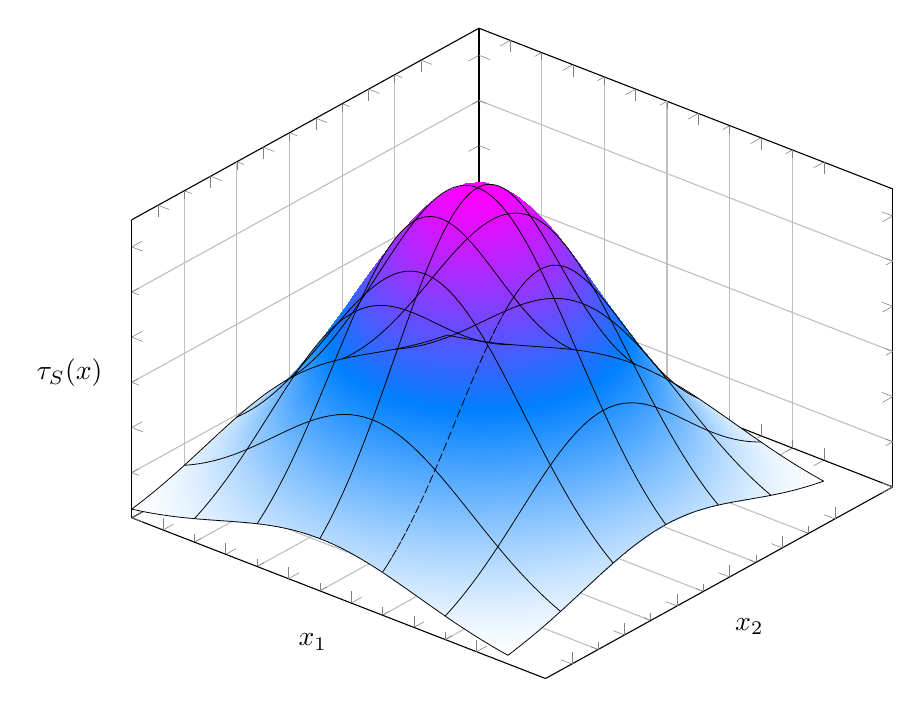
\begin{tikzpicture}
     \begin{axis}[
            view={40}{40},
          %x dir=reverse,
          %y dir=reverse,
          width=320pt,
          height=280pt,
          mesh,
          colormap/cool,
          %mesh/ordering=x varies,
          z buffer=auto,%reverse xy seq,
          xmin=-0.5,xmax=5.5,
          ymin=-0.5,ymax=5.5,
          zmin=0,zmax=0.3,
          enlargelimits=upper,
          xtick=data,
          extra tick style={grid=major},
          ytick={0,...,5},xtick={0,...,5},
          grid=minor,
          xticklabels=\empty,
          yticklabels=\empty,
          zticklabels=\empty,
          xlabel={$x_1$},
          ylabel={$x_2$},
          zlabel={$\tau_S(x)$},
          zlabel style={rotate=-90},
          minor tick num=1,
          samples=70]
        \addplot3[surf, domain=-0.5:5.5, shader=interp] {0.35*(exp(-0.2*(x-2.5)*(x-2.5)-0.2*(y-2.5)*(y-2.5))};
        \foreach \xx in {-0.5,0.5,...,5.5}
        {
          \addplot3+[domain=-0.5:5.5, line width=0.1mm, mark=none, color=black, samples y=0]
           ({\xx}, {x}, {0.35*(exp(-0.2*(\xx-2.5)*(\xx-2.5)-0.2*(x-2.5)*(x-2.5))});
        }
  
        % y=constant grids lines
        \foreach \yy in {-0.5,0.5,...,5.5}
        {
           \addplot3[domain=-0.5:5.5, line width=0.1mm, mark=none, color=black, samples y=0]
           ({x}, {\yy}, {0.35*(exp(-0.2*(x-2.5)*(x-2.5)-0.2*(\yy-2.5)*(\yy-2.5))});
        }
  
  
     \end{axis}
  \end{tikzpicture}
  \vspace*{2px}
  \caption[Example of an arbitrary mass-energy density]{An example of an arbitrary mass-energy density $\tau_S$ plotted against two dimensions $x_1$ and $x_2$ belonging to the hypersurface $S$. }\label{tauSexample}
  \end{figure}

  \begin{figure}[ht!]
    \captionsetup{justification=justified}
    \centering
    
    \pgfmathsetmacro{\gconv}{2*326.32446}
    % from https://tex.stackexchange.com/a/435234/121799
    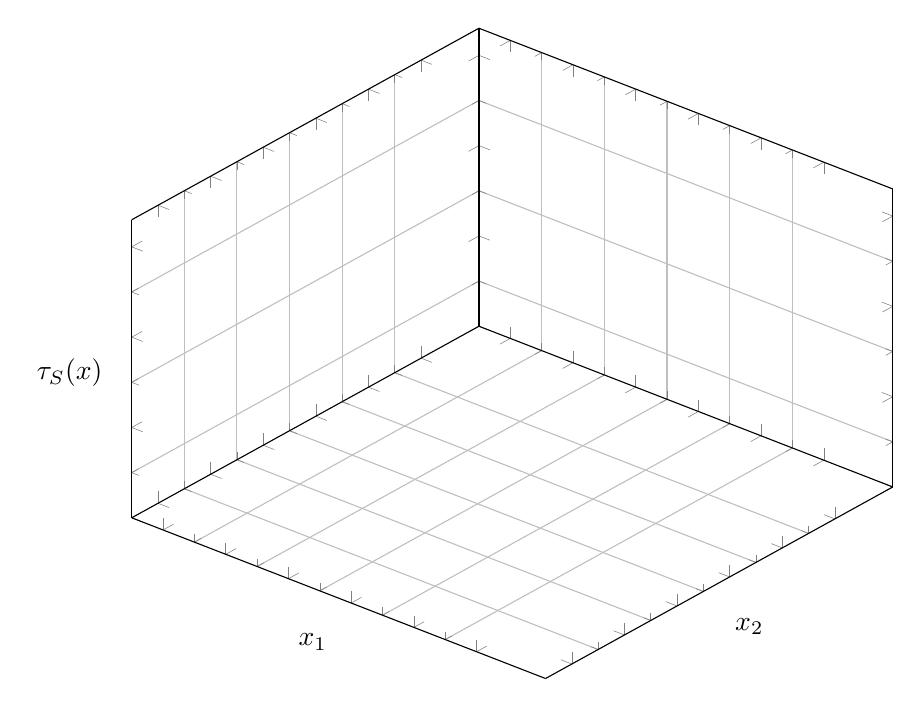
\begin{tikzpicture}[declare function={% (0.00001*\n!/(0.01*\x!*0.01*\y!*0.01*(\n-\x-\y)!))*
    f(\x,\y,\px,\py,\n)=(0.000001*\n!/(0.01*\x!*0.01*\y!*0.01*(\n-\x-\y)!))*pow(\px,\x)*pow(\py,\y)*pow(1-\px-\py,\n-\x-\y);}] % 
    \pgfplotsset{set layers}
    \begin{axis}[% from section 4.6.4 of the pgfplotsmanual
            view={40}{40},
            %x dir=reverse,
            %y dir=reverse,
            width=320pt,
            height=280pt,
            mesh,
            %mesh/ordering=x varies,
            z buffer=auto,%reverse xy seq,
            xmin=-0.5,xmax=5.5,
            ymin=-0.5,ymax=5.5,
            zmin=0,zmax=0.3,
            enlargelimits=upper,
            xtick=data,
            extra tick style={grid=major},
            ytick={0,...,5},xtick={0,...,5},
            grid=minor,
            xticklabels=\empty,
            yticklabels=\empty,
            zticklabels=\empty,
            xlabel={$x_1$},
            ylabel={$x_2$},
            zlabel={$\tau_S(x)$},
            zlabel style={rotate=-90},
            minor tick num=1,
            ]
    
      \addplot3 [point meta=0,visualization depends on={
      \gconv*z \as \myz}, % you'll get told how to adjust the prefactor
      scatter/@pre marker code/.append style={/pgfplots/cube/size z=\myz},%
      scatter/@pre marker code/.append style={/pgfplots/cube/size x=24.3018pt},%
      scatter/@pre marker code/.append style={/pgfplots/cube/size y=21.71275pt},%
      scatter,only marks,
      mark=my cube*,mark size=5,opacity=1,domain=0:5,domain y=0:5,samples=6,samples y=6]
      {0.35*(exp(-0.2*(x-2.5)*(x-2.5)-0.2*(y-2.5)*(y-2.5))};
        \end{axis}
    \end{tikzpicture}
    \vspace*{2px}
    \caption[Approximated arbitrary mass-energy density]{Here, the arbitrary mass-energy density $\tau_S$ depicted in figure \ref{tauSexample} has been approximated by a function which is constant in each mesh cell.}\label{tauSapprox}
    \end{figure}
    We can then suppose that with a suitably fine mesh\label{meshref} on $S$,\footnote{Note that the mesh is only a mesh in $S$, so the cells of the mesh are cube-like subsets of $S$. The time might not be constant across each cell because of the possible curvature of $S$.} any mass energy density $\tau_S(x)$ (e.g. such as the one depicted in figure \ref{tauSexample}) can be approximated to a function (e.g. like the one depicted in figure \ref{tauSapprox}) that has constant values on each cell of this mesh and such that the approximation value at a cell belongs to a finite pool of possible values. For instance, if $c_x$ is the cell which contains $x\in S$, and $\tau_{\text{max}}$ is the maximum possible value the mass-energy density could be, then we could define the approximation to $\tau_S(x)$ at cell $c_x$ to be
    \begin{equation}\label{tauapproxformula}
    \tau_S(c_x)=\frac{\tau_{\text{max}}}{N}\floor*{N\Big(\frac{\text{average of }\tau_S\text{ over }c_x}{\tau_{\text{max}}}\Big)+0.5}
    \end{equation}
    where $\floor*{z}$ is the biggest integer $n\leq z$, and where $N$ is a fixed large number. Then $\tau_S(c_x)$ will have $N+1$ possible values between $0$ and $\tau_{\text{max}}$.  There will then only need to be a countable number of approximations $\tau_{S,i}$ to approximate any arbitrary mass-energy density $\tau_S$ on $S$.  As long as we choose the cells in the mesh to be sufficiently small and $N$ to be sufficiently large, we can describe physical reality up to our desired level of accuracy. Thus, we assume that for each of the countable states in the orthonormal basis $\{\ket*{\Gamma_{i}}:i\in\mathbb{N}\}$, there will be a corresponding function $\tau_{S,i}$ defined on $S$ which is constant on every cell of $S$ and in which 
\begin{equation}\label{approxeigen}
\hat{T}_S(c_x)\ket*{\Gamma_{i}}= \tau_{S,i}(c_x)\ket*{\Gamma_{i}}
\end{equation} 
for all $x\in S$ where $ \tau_{S,i}(c_x)= \tau_{S,i}(x)$ and where $\hat{T}_S(c_x)$ is the observable corresponding to the average approximated value of the physical quantity $T_S(x)$ over the cell $c_x$ (approximated as in (\ref{tauapproxformula}) with $\tau_S$ replaced by $T_S$), but we will normally just write
\begin{equation}\label{approxeigen2}
  \hat{T}_S(x)\ket*{\Gamma_{i}}= \tau_{S,i}(x)\ket*{\Gamma_{i}}
  \end{equation}
with the implicit understanding that by (\ref{approxeigen2}) we really mean (\ref{approxeigen}), and that when we speak of $\ket*{\Gamma_{i}}$ and $\tau_{S,i}$ as simultaneous $\hat{T}_S$-eigenstates and simultaneous $\hat{T}_S$-eigenvalues respectively, we implicitly understand $\hat{T}_S$ and $\tau_{S,i}$ to be defined over cells of the form $c_x\subset S$ rather than over spacetime locations $x\in S$.

Now the additional variables beyond standard quantum theory that are included in Kent's theory are given by one of these simultaneous $\hat{T}_S$-eigenvalues $\tau_{S,i}$ that (approximately) describe a possible outcome for a mass-energy density measurement over the whole of $S$. We will let $\tau_S$ denote the particular  $\tau_{S,i}$ that constitute the additional variables of Kent's theory. 

Now the particular density $\tau_S$ which is found to describe $S$ can't be absolutely anything. Limitations are placed on what $\tau_S$ can be, and these limitations will depend on the initial conditions of Kent's theory. Kent assumes that all physics that we wish to describe takes place between two hypersurfaces $S_0$ %
\nomenclature{$S_0$}{Initial hypersurface for which Kent assumes all physics occurs between $S_0$ and $S$, \nomrefpage}%
 and $S$, with $S_0$ much earlier than $S$ so that $S_0$ and $S$ don't intersect. Initial conditions are determined on the hypersurface $S_0$ so that we can assume it is described by a state $\ket*{\Psi_0}\in H_{S_0}$ in the Tomonaga-Schwinger picture. %
 \nomenclature{$\ket*{\Psi_0}$}{The state of the initial hypersurface $S_0$ in the Tomonaga-Schwinger picture, \nomrefpage}% 
 If we  define 
\begin{equation}\label{SchwingerUnitaryOP}
U_{SS_0}=U[S]U[S_0]^{-1},
\end{equation} 
where $U[S]$ and $U[S_0]$ are the Schwinger unitary operators introduced on
 page \pageref{SchwingerOperator}, then
 given the state $\ket*{\Psi_0}$, there will be a corresponding state $\ket*{\Psi_S}=U_{SS_0}\ket*{\Psi_0}\in H_S$  %
 \nomenclature{$\ket*{\Psi_S}$}{The state $U_{SS_0}\ket*{\Psi_0}\in H_S$ in the Tomonaga-Schwinger picture, \nomrefpage}%
  that describes the hypersurface $S$ in the Tomonaga-Schwinger picture. Figure \ref{S1} depicts the evolution of the state $\ket*{\Psi_0}$ to the state $\ket*{\Psi_S}$.
  \begin{figure}[ht!]
    \captionsetup{justification=justified}
    \centering
    
    \tikzmath{
    \a= 1;  
    \h=-1;
    \md = (\a+\h)/2;
    \lrange = 4;
    \rrange=2;
    \fictlabel=(\rrange-\lrange)/2;
    \tlen=0.75;
    \labelpos=(-\lrange-\a)/2;
    } 
    
    \begin{tikzpicture}[thick, scale=2]
    \def\dotsize{0.7}
    \definecolor{tempcolor}{RGB}{0,151,76}
    \draw[<->] (-\lrange, \h) node[left] {$S_0$} -- (\rrange, \h) node[right] {$S_0$};
    \draw[<->](-\lrange, \a) node[left] {$S$} --  (\rrange, \a)  node[right] {$S$};                   
    \draw[->] (\rrange,\md-\tlen/2) --  (\rrange,\md+\tlen/2) node[midway,right]{time}; 
    \coordinate[label = above: Notional Measurement of $T_S(x)$ on $S$]  (D) at (\fictlabel,\a+0.2); 
    \node (start) at (\labelpos,\h) [below] {Initial State $\ket*{\Psi_0}$};
    \node (final) at (\labelpos,\a) [below] {Unitary Evolution $\ket*{\Psi_S}=U_{SS_0}\ket*{\Psi_0}$};
    \draw [->, shorten <= 5pt] (start) [above] -- (final); 
    
    \end{tikzpicture}
    
    \vspace*{2px}
    \caption[Depiction of a notional measurement of $T_S(x)$]{A notional measurement of $T_S(x)$ is made for all $x\in S$. The simultaneous  $\hat{T}_S$-eigenstate $\ket*{\Gamma}$ with $\hat{T}_S(x)\ket*{\Gamma}=\tau_S(x)\ket*{\Gamma}$ is selected with probability $\abs{\mel{\Gamma}{U_{SS_0}}{\Psi_0}}^2$ $=\abs{\ip{\Gamma}{\Psi_S}}^2$. The values $\tau_S(x)$ obtained for $T_S(x)$ are then used to calculate the physical properties at the spacetime location $y$.  }
    \label{S1}
    \end{figure} Then if $\ket*{\Gamma}$ is a simultaneous  $\hat{T}_S$-eigenstate with $\hat{T}_S(x)\ket*{\Gamma}=\tau_S(x)\ket*{\Gamma}$, then the probability $P(\Gamma|\Psi_0)$ %
  \nomenclature{$P(\Gamma|\Psi_0)$}{The probability that  $S$ will be found to be in the state $\ket*{\Gamma}$ with mass-energy density $\tau_S(x)$ given that $S_0$ was initially in the state $\ket*{\Psi_0}$, see equation (\ref{bornrule}), \nomrefpage}%
  that $S$ will be found to be in the state $\ket*{\Gamma}$ given the initial state $\ket*{\Psi_0}$ describing $S_0$ will be given by the Born Rule (see page \pageref{bornrule}):    
  \begin{equation}\label{bornpsi}
    P(\Gamma|\Psi_0) = \abs{\mel{\Gamma}{U_{SS_0}}{\Psi_0}}^2=\abs{\ip{\Gamma}{\Psi_S}}^2
    \end{equation}
  It's  possible that there could be more than one simultaneous  $\hat{T}_S$-eigenstate  in  $H_S$ that has the simultaneous  $\hat{T}_S$-eigenvalue $\tau_S$, but it is the mass-energy density $\tau_S$ itself rather than one of the eigenstates with mass-energy density $\tau_S$ that constitute the additional variables that Kent adds to standard quantum theory. 

{\interfootnotelinepenalty=10000   Also note that  if every simultaneous $\hat{T}_S$-eigenstate $\ket*{\Gamma}$ with simultaneous $\hat{T}_S$-eigenvalue $\tau_S$ satisfies $\abs{\mel{\Gamma}{U_{SS_0}}{\Psi_0}}=0$, then by (\ref{bornpsi}), $\tau_S$ will have zero probability, and hence, it will not be a possible measurement outcome for $T_S$ given $\ket*{\Psi_0}$.\footnote{\label{discreteRV}When dealing with continuous random variables, if the probability of the random variable having a particular value is  zero, it does not follow that it is impossible for the random variable to have this value. However, in the case of discrete random variables,  if the probability of the random variable having a particular value is  zero, then it does  follow that it is impossible for the random variable to have this value. Because we are using (\ref{tauapproxformula}) to approximate the energy density, we can treat  $T_S$ as a discrete random variable, hence the claim that if $T_S=\tau_S$ has zero probability,  then $\tau_S$ will not be a possible measurement outcome for $T_S$ given $\ket*{\Psi_0}$.} It is for this reason that we can't expect the measurement outcome of $T_S$ on $S$ to be absolutely anything.}










 







